% !TEX root = /media/ueslei/Ueslei/INPE/PCI/Projetos/Guia_COAWST/main.tex
\chapterimage{header.jpg}
\chapter{Building the WRF}\index{Construindo o WRF}
\bigskip 
\noindent Now that we have learned how to simulate a test case and change the coupling rate and number of processors, we will begin 
the process of creating a specific grid and the initial and boundary conditions for the WRF using the NCEP Climate Forecast System Reanalysis (CFSR; \cite{Saha2006}).
\bigskip

\section{Compiling WRF in Kerana cluster}
\bigskip
\noindent It is recommended to copy the WRF folder inside COAWST to your work root area, in order to avoid conflicts
if you choose to use the WRF without coupling to the COAWST model. Therefore:\bigskip

\begin{bashcode}
cd /scratch/name.surname/COAWST
cp -r WRF /scratch/nome.dsobrenome
\end{bashcode}
\bigskip

\noindent Activate the modules in the \textit{setup\_pgi.sh} file with the command:
\bigskip
\begin{bashcode}
source setup_pgi.sh
\end{bashcode}
\bigskip

\noindent Enter the copy folder of the WRF (\textit{/home/name.surname/WRF}) and run:
\bigskip

\begin{bashcode}
./configure
\end{bashcode}
\bigskip

\begin{tcolorbox}[enhanced,
  grow to left by=0cm,%   equivalent to negative mdframed 'leftmargin'
  grow to right by=0cm,%  equivalent to negative mdframed 'rightmargin'
  enlarge top by=0cm,%     equivalent to mdframed 'skipabove'
  enlarge bottom by=0cm,%  equivalent to mdframed 'skipbelow'
  tcbox raise base,
  boxrule=1.0pt,
  left=18mm,
  colframe=red!50!black,coltext=red!25!black,colback=red!10!white,
  overlay={\begin{tcbclipinterior}\fill[red!75!blue!50!white] (frame.south west)
    rectangle node[text=white,font=\sffamily\bfseries\footnotesize,rotate=0] {WARNING} ([xshift=18mm]frame.north west);\end{tcbclipinterior}}]
The next step can be automated. If you choose the automated compilation, see Section \textcolor{bleu_cite}{\ref{autowrf}}.
\end{tcolorbox}
\bigskip

\noindent If you have automated the compilation process, as shown in Section \textcolor{bleu_cite}{\ref{autowrf}}, the files \textit{real.exe}, \textit {wrf.exe},
\textit{tc.exe} and \textit{ndown.exe} will be created. If you choose the manual option on the Kerana cluster, look down for the option \textit{Cray XC CLE / Linux x86 \_64, Cray compiler with gcc (dmpar)}.
\bigskip

\noindent In the next option, the following message will appear:
\bigskip

\begin{bashcode}
Compile for nesting? (1=basic, 2=preset moves, 3=vortex following) [default 1]:
\end{bashcode}
\bigskip

\noindent Choose option 1.
\bigskip

\begin{tcolorbox}[enhanced,
  grow to left by=0cm,%   equivalent to negative mdframe 'leftmargin'
  grow to right by=0cm,%  equivalent to negative mdframed 'rightmargin'
  enlarge top by=0cm,%     equivalent to mdframed 'skipabove'
  enlarge bottom by=0cm,%  equivalent to mdframed 'skipbelow'
  tcbox raise base,
  boxrule=1.0pt,
  left=18mm,
  colframe=red!50!black,coltext=red!25!black,colback=red!10!white,
  overlay={\begin{tcbclipinterior}\fill[red!75!blue!50!white] (frame.south west)
    rectangle node[text=white,font=\sffamily\bfseries\footnotesize,rotate=0] {WARNING} ([xshift=18mm]frame.north west);\end{tcbclipinterior}}]
End of the automated build process.
\end{tcolorbox}
\bigskip

\noindent Type:
\bigskip

\begin{bashcode}
compile em_real
\end{bashcode}
\bigskip

\noindent The \textit{real.exe}, \textit{wrf.exe}, \textit{tc.exe} and \textit{ndown.exe} will be generated in the \textit{/home/name.surname/WRF/test/em\_real}.
\bigskip

\section{WRF Preprocessing System (WPS)}\label{wpssecao}
\bigskip

\noindent To build the initial and boundary conditions of the WRF, we will use WRF Preprocessing System (WPS). The WPS is a set of three programs that 
prepare the input data for the simulations. It consists of the following modules:
\bigskip

\begin{itemize}
\item \textbf{\textit{geogrid}}: Defines the model domain and interpolates the geographic data for the grid;
\item \textbf{\textit{ungrib}}: Extract weather fields from \textit{.grib} files;
\item \textbf{\textit{metgrid}}: Interpolates the weather fields extracted by ungrib to the model grid defined by metrid.
\end{itemize}
\bigskip

\noindent WPS is controlled by the \textit{namelist.wps} file and is outlined in Figure \textcolor{bleu_cite}{\ref{wpsdetalha}}.
\bigskip

\noindent You can find more information in the WPS 
\textcolor{bleu_cite}{\textit{website}\footnote{\textcolor{bleu_cite}{\href{http://www2.mmm.ucar.edu/wrf/OnLineTutorial/}{http://www2.mmm.ucar.edu/wrf/OnLineTutorial/}}}}.
\bigskip

\noindent After creating these files, the \textit{real.exe} is used to interpolate the meteorological fields to \texteta level.
\bigskip

\begin{figure}[H]
    \centering
    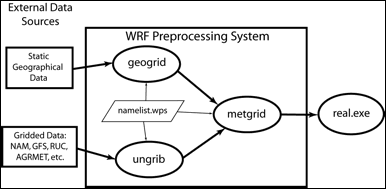
\includegraphics[width=0.65\textwidth]{image002.png}
    \caption{WPS schemeatic. \newline Author: \textcite{duda2006}.}
    \label{wpsdetalha}
\end{figure}
\bigskip

\subsection{Downloading WPS}
\bigskip

\noindent WPS is included in the COAWST package, however WPS can be downloaded by visiting it
\textcolor{bleu_cite}{\textit{website}\footnote{\textcolor{bleu_cite}{\href{http://www2.mmm.ucar.edu/wrf/users/download/get\_source.html}{http://www2.mmm.ucar.edu/wrf/users/download/get\_source.html}}}}. 
Download it and add the \textit{tar.gz} file inside the cluster with \textit{sftp}:
\bigskip

\begin{bashcode}
sftp -P2000 name.surname@acesso-hpc.cptec.inpe.br
cd COAWST
put WPSV3.9.0.1.tar.gz
\end{bashcode}
\bigskip

\noindent To unzip, use \textit{ssh} to enter the cluster and type:
\bigskip

\begin{bashcode}
ssh -Y name.surname@acesso-hpc.cptec.inpe.br -p 2000
cd COAWST
tar -xvzf WPSV3.9.0.1.tar.gz
\end{bashcode}
\bigskip

\subsection{Compiling WPS in the Kerana cluster}\label{wpsker}
\bigskip

\begin{tcolorbox}[enhanced,
    grow to left by=0cm,%   equivalent to negative mdframed 'leftmargin'
    grow to right by=0cm,%  equivalent to negative mdframed 'rightmargin'
    enlarge top by=0cm,%     equivalent to mdframed 'skipabove'
    enlarge bottom by=0cm,%  equivalent to mdframed 'skipbelow'
    tcbox raise base,
    boxrule=1.0pt,
    left=18mm,
    colframe=red!50!black,coltext=red!25!black,colback=red!10!white,
    overlay={\begin{tcbclipinterior}\fill[red!75!blue!50!white] (frame.south west)
      rectangle node[text=white,font=\sffamily\bfseries\footnotesize,rotate=0] {WARNING} ([xshift=18mm]frame.north west);\end{tcbclipinterior}}]
      As stated earlier in Section \textcolor{bleu_cite}{\ref{wpsker}}, WPS is included with COAWST. We recommend to use this version.
\end{tcolorbox}
\bigskip

\noindent To compile the WPS and generate the executables, it is necessary to activate the libraries with \textit{setup\_pgi.sh},
found in the directory \textit{/home/name.surname/repository}. Activate them with the command:
\bigskip

\begin{bashcode}
source setup_pgi.sh
\end{bashcode}
\bigskip

\noindent Inside the WPS folder, enter the following command:
\bigskip

\begin{bashcode}
./configure
\end{bashcode}
\bigskip

\noindent You will be asked which machine and compiler will be used. Choose the option 
\textit{Cray XE / XC CLE / Linux x86 \_64, PGI compiler (serial)}. In this case, a message will be generated that Fortran is not compatible 
with C and NetCDF, but ignore it.
\bigskip

\noindent Open \textit{configure.wps} file:
\bigskip

\begin{bashcode}
nedit configure.wps
\end{bashcode}
\bigskip

\noindent Modify:
\bigskip

\begin{bashcode}
WRF_DIR  = ../WRFV3
SFC      = ftn
SCC      = gcc
DM_CC    = cc
DM_FC    = ftn
FFLAGS   = -N255 -f free -h byteswapio
F77FLAGS = -N255 -f fixed -h byteswapio

\end{bashcode}
\bigskip

\noindent By:
\bigskip

\begin{bashcode}
WRF_DIR  = /scratch/name.surname/WRF
SFC      = ftn
SCC      = gcc
DM_CC    = gcc
DM_FC    = ftn
FFLAGS   =
F77FLAGS =
\end{bashcode}
\bigskip

\noindent Save the changes and start the compilation with the command:
\bigskip

\begin{bashcode}
./compile
\end{bashcode}
\bigskip

\noindent You should generate the executables \textit{metgrid.exe} and \textit{geogrid.exe}. However, it is possible that \textit{ungrib.exe} 
is not generated. In this case, repeat:
\bigskip

\begin{bashcode}
./configure
\end{bashcode}
\bigskip

\noindent Choose the option \textit{Linux x86\_64, PGI compiler (dmpar)}.
\bigskip

\noindent Open \textit{configure.wps} file again, modify:
\bigskip

\begin{bashcode}
WRF_DIR = ../WRFV3
SFC     = pgf90
SCC     = pgcc
DMFC    = mpif90
DMCC    = mpicc
\end{bashcode}
\bigskip

\noindent By:
\bigskip

\begin{bashcode}
WRF_DIR = /home/name.surname/WRF
SFC     = ftn
SCC     = gcc
DMFC    = ftn
DMCC    = gcc
\end{bashcode}
\bigskip

\noindent The installer will generate only the \textit{ungrib.exe}.

\section{Building your project using CFSR}
\bigskip

\noindent NCEP Climate Forecast System Reanalysis 
\textcolor{bleu_cite}{\textit{CFSR})\footnote{\textcolor{bleu_cite}{\href{http://rda.ucar.edu/datasets/ds093.0}{http://rda.ucar.edu/datasets/ds093.0}}}}
a reanalysis, avaliable from January 1979 to December 2010, with a coupled model (atmosphere-ocean-land surface and sea ice) that
assimilates orbital data, research cruises, oceanographic buoys and weather stations. This database
has vertical resolution with 38 levels, extending from the surface to 1 hPa, with a 6-hour temporal resolution
and horizontal of 0.5\degree for pressure levels data and 0.312\degree for variables on the surface.
\bigskip

\noindent To access the data it is necessary to register on the site. After, access the database link,
click on the\textit{Data Acess} and then, \textit{Get a subset}.
\bigskip

\noindent On the next page, as seen in Figure \textcolor{bleu_cite}{\ref{detalhacfsr}}, write the temporal selection,
and select in \textit {Parameter presets} one of the three parameters of the WRF presets: (\textit{Pressure},
\textit{Surface} and \textit{SST}). 
\bigskip

\begin{tcolorbox}[enhanced,
    grow to left by=0cm,%   equivalent to negative mdframed 'leftmargin'
    grow to right by=0cm,%  equivalent to negative mdframed 'rightmargin'
    enlarge top by=0cm,%     equivalent to mdframed 'skipabove'
    enlarge bottom by=0cm,%  equivalent to mdframed 'skipbelow'
    tcbox raise base,
    boxrule=1.0pt,
    left=18mm,
    colframe=red!50!black,coltext=red!25!black,colback=red!10!white,
    overlay={\begin{tcbclipinterior}\fill[red!75!blue!50!white] (frame.south west)
      rectangle node[text=white,font=\sffamily\bfseries\footnotesize,rotate=0] {WARNING} ([xshift=18mm]frame.north west);\end{tcbclipinterior}}]
      Only one parameter (\textit{Pressure}, \textit{Surface} and \textit{SST}) can be downloaded at a time, therefore you need to repeat this step three times.
\end{tcolorbox}
\bigskip

\begin{figure}[H]
    \centering
    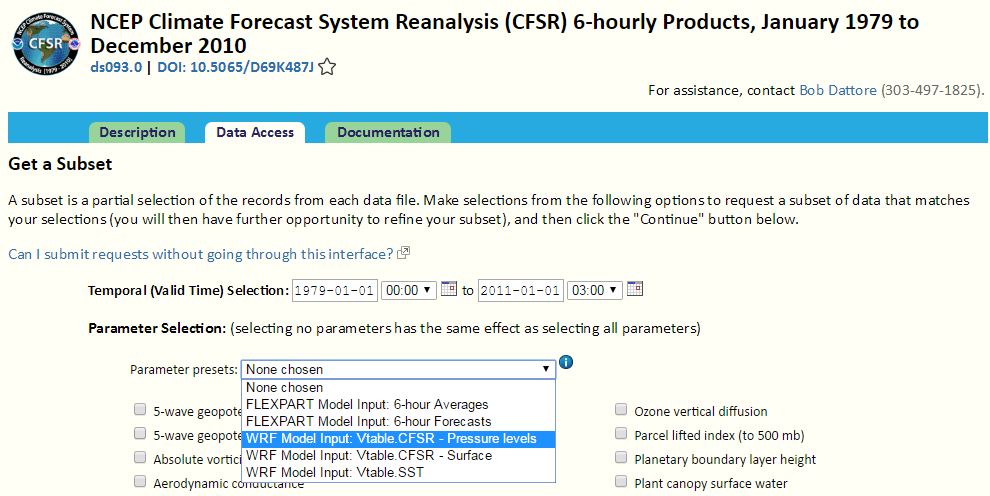
\includegraphics[width=0.95\textwidth]{1.png}
    \caption{Screenshot of the CFSR data page.}
    \label{detalhacfsr}
\end{figure}
\bigskip

\noindent Download the data (as \textit{GRIB}) and separate it into three folders according to the parameters of each one:
SST, Surface and Pressure. Compress them and put them in the cluster:
\bigskip

\begin{bashcode}
tar -cvzf SST.tar.gz SST/
tar -cvzf Pressure.tar.gz Pressure/
tar -cvzf Surface.tar.gz Surface/
ssh -Y name.surname@acesso-hpc.cptec.inpe.br -p 2000
mkdir Data_CFSR
exit
sftp -P2000 name.surname@acesso-hpc.cptec.inpe.br
cd Data_CFSR
put SST.tar.gz
put Pressure.tar.gz
put Surface.tar.gz
exit
ssh -Y name.surname@acesso-hpc.cptec.inpe.br -p 2000
cd Data_CFSR
tar -xvzf SST.tar.gz
tar -xvzf Pressure.tar.gz
tar -xvzf Surface.tar.gz
\end{bashcode}
\bigskip

\subsection{\textit{geogrid}}\label{geowps}
\bigskip

\noindent As previously mentioned, \ textit {geogrid} generates the grid domain using geographic data. The data can be obtained from it 
\textcolor{bleu_cite}{\textit{website}\footnote{\textcolor{bleu_cite}{\href{http://www2.mmm.ucar.edu/wrf/users/download/get\_sources\_wps\_geog.html}{http://www2.mmm.ucar.edu/wrf/users/download/get\_sources\_wps\_geog.html}}}}
, or directly from the repository guide:
\bigskip

\begin{bashcode}
/scratch/name.surname/repositorio/COAWST/WPS/geog
\end{bashcode}
\bigskip

\noindent With the CFSR and \textit{geogrid} data in hand, enter into the WPS directory and open \textit{namelist.wps}. 
The file structure is shown in Figure \textcolor{bleu_cite}{\ref{namelistwps}}:
\bigskip

\begin{bashcode}
nedit namelist.wps
\end{bashcode}
\bigskip

\begin{figure}[H]
    \centering
    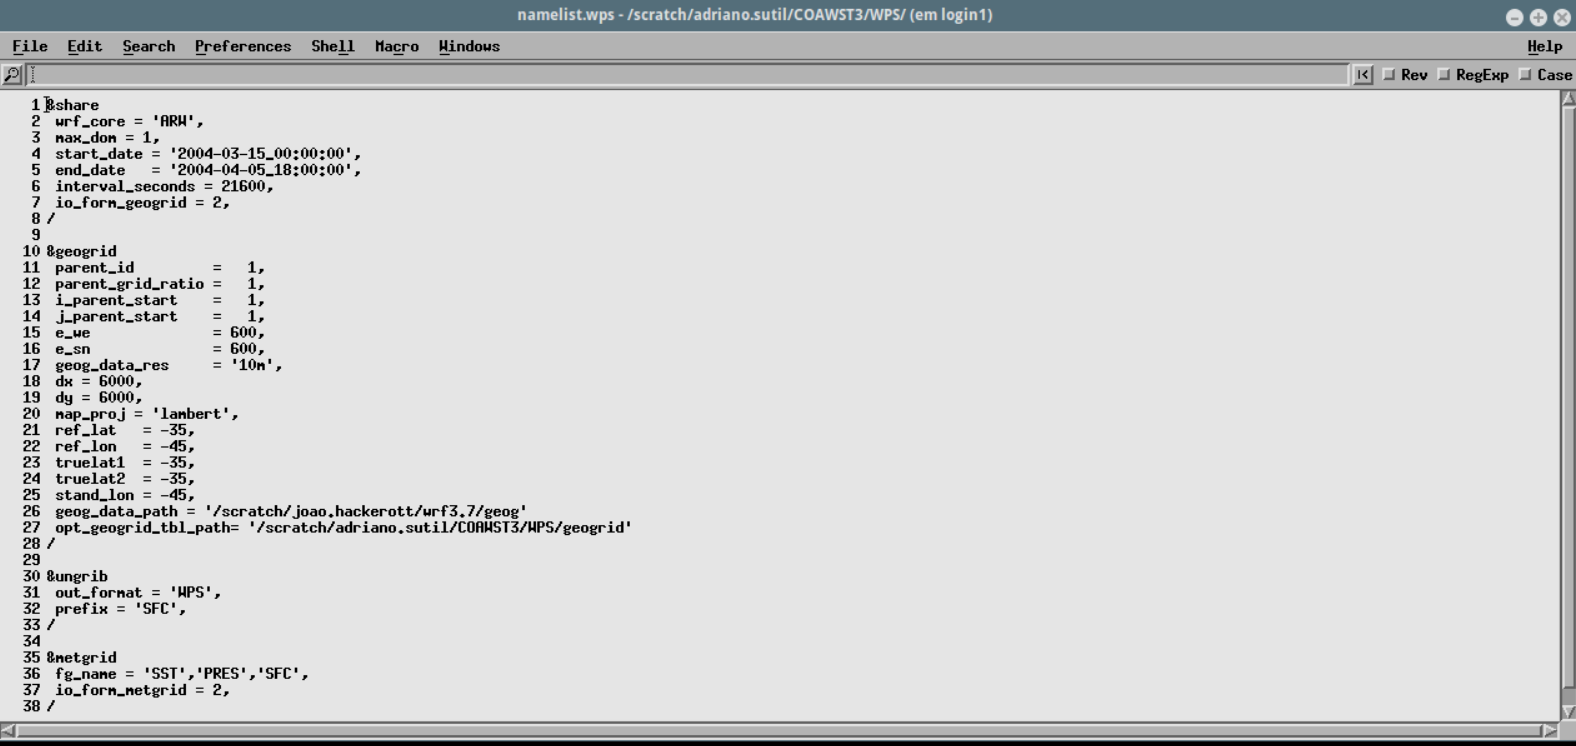
\includegraphics[width=0.95\textwidth]{image3411.png}
    \caption{\textit{namelist.wps} example.}
    \label{namelistwps}
\end{figure}
\bigskip

\noindent Change the \textit{geog\_data\_path} path to the directory where geographic data is located (\textit{geog folder}), 
\textit{geog\_data\_res} if you want to use other geographic data and \textit{opt\_geogrid\_tbl\_path}, which is the 
\textit{geogrid} directory.

\bigskip

\noindent The WPS uses a ground zero point defined by the user as the latitude and longitude degrees in \textit{ref\_lat} and \textit{ref\_lon}.
It will generate the grid from that point and through the chosen spatial resolution. Take as example the Figure
\textcolor{bleu_cite}{\ref{namelistwps}}: a simulation will be prepared with 6 km of spatial resolution (\textit{dx} and \textit{dy} = 6000),
in Lambert projection, with 600 grid points. Using as reference latitude -35\degree longitude -45\degree, a grid will be created with 
600 points in the west-east direction (\textit{e\_we}) and 600 points in the south-north direction (\textit{e\_sn}), with each
point having a spacing of 6000 meters (6 km) between them.
\bigskip

\noindent To start \textit{geogrid}, you need a file with a Shell extension (\textit{.sh}), which submits program to be executed in the cluster.
 It can be found in the \textit{/repository/WPS\_scripts} directory. Move the contents of the folder to the WPS directory with the commands:
\bigskip

\begin{bashcode}[fontsize=\footnotesize]
cd /home/name.surname/repositorio/WPS_scripts
mv qsub_geogrid.sh qsub_ungrib.sh qsub_metgrid.sh /home/name.surname/COAWST/WPS
\end{bashcode}
\bigskip

\noindent The structure of the \textit{qsub\_geogrid.sh} file is shown in Figure \textcolor{bleu_cite}{\ref{qsubgeonedit}}. 
Modify the directory according to your user.
\bigskip

\begin{figure}[H]
    \centering
    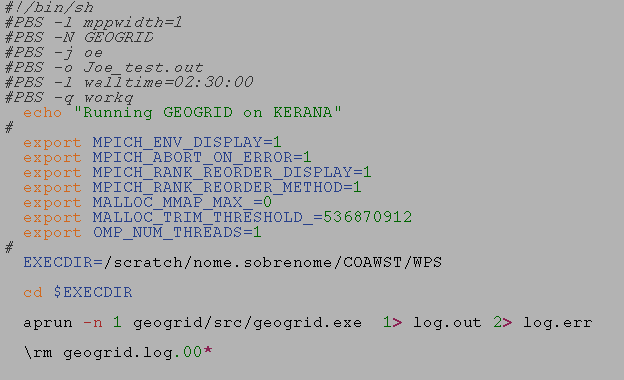
\includegraphics[width=0.95\textwidth]{qsubgeonedit.png}
    \caption{\textit{qsub\_geodrid.sh} example.}
    \label{qsubgeonedit}
\end{figure}
\bigskip

\noindent To run \textit{geogrid}, use \textit{qsub} command:
\bigskip

\begin{bashcode}
qsub qsub_geodrid.sh
\end{bashcode}
\bigskip

\noindent Two files will be generated: \textit{log.err} e \textit{log.out}. you can follow how the program is being executed and search for errors. 
The program completion message is showned in Figure \textcolor{bleu_cite}{\ref{qsubgeofinal}}, in the file \textit{log.out}.

\bigskip

\begin{figure}[H]
    \centering
    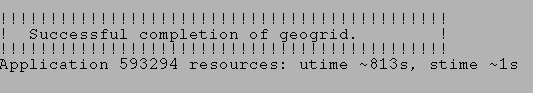
\includegraphics[width=0.55\textwidth]{qsubgeo.png}
    \caption{Example of completion of \textit{geogrid}.}
    \label{qsubgeofinal}
\end{figure}
\bigskip

\noindent When completing the execution of \textit{geogrid}, the file \textit{geo\_em\_d01.nc} will be generated.
 You can view the NetCDF file with Ncview:
\bigskip

\begin{bashcode}
module load netcdf
ncview geo_em_d01.nc
\end{bashcode}
\bigskip

\noindent You will always need to run \textit{geogrid} until you find a domain that is suitable for your project, 
since WPS does not have a graphical interface. One solution to work around the problem is to use NCAR Command Language version 6.4 
(NCL; \cite{Ncl2017}) to plot the image of the chosen domain. This will be the subject of the next subsection.

\bigskip

\subsection{Using the NCL to plot the grid domain}
\bigskip

\noindent To install the NCL, move the \textit{NCL} folder inside the repository:
\bigskip

\begin{bashcode}
mv /scratch/name.surname/repositorio/NCL /scratch/name.surname
\end{bashcode}
\bigskip

\noindent Open the \textit{.bashrc} file:
\bigskip

\begin{bashcode}
cd
nedit .bashrc
\end{bashcode}
\bigskip

\noindent Add the following command lines, changing to your username:
\bigskip

\begin{bashcode}
export NCARG_ROOT=/scratch/name.surname/NCL
export PATH=$NCARG_ROOT/bin:$PATH
\end{bashcode}
\bigskip

\noindent Save the file, reload the modules inside \textit{.bashrc} and then execute NCL.
\bigskip

\begin{bashcode}
source .bashrc
ncl
\end{bashcode}
\bigskip

\noindent Check if the NCL has been initialized as in Figure \textcolor{bleu_cite}{\ref{nclinit}}.
\bigskip

\begin{figure}[H]
    \centering
    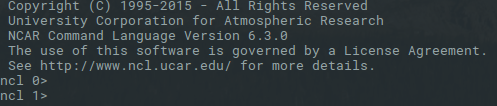
\includegraphics[width=0.95\textwidth]{nclinit.png}
    \caption{Example of NCL initialization.}
    \label{nclinit}
\end{figure}
\bigskip


\noindent Enter the repository and open the \textit{plotgrids.ncl} file. 
This script generates the domain image from the data in the \textit{namelist.wps} file.
\bigskip

\begin{bashcode}
cd /scratch/name.surname/repositorio
nedit plotgrids.ncl
\end{bashcode}
\bigskip

\noindent Modify the \textit{namelist.wps} directory according to your user area:
\bigskip

\begin{bashcode}
filename = "/home/name.surname/COAWST/WPS/namelist.wps"
\end{bashcode}
\bigskip

\noindent Run the code with the command:
\bigskip

\begin{bashcode}
ncl plotgrids.ncl
\end{bashcode}
\bigskip

\noindent The code will search for the grid points and the domain resolution through the file \textit{namelist.wps} and show it on the screen, 
as shown in Figure \textcolor{bleu_cite}{\ref{nclgrids}}. Repeat the process until you find a domain that suits your needs.
\bigskip

\begin{figure}[H]
    \centering
    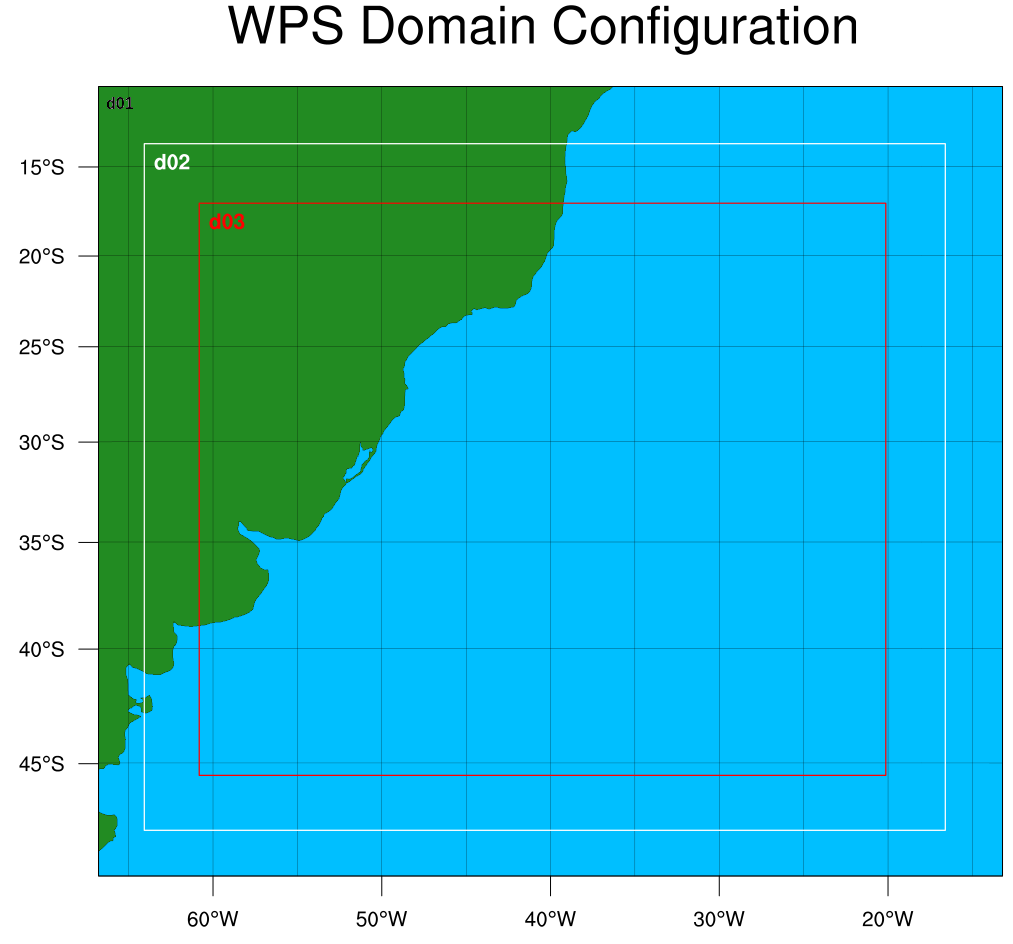
\includegraphics[width=0.65\textwidth]{wps_domain_new.png}
    \caption{Figure generated by the \textit{plotgrids.ncl} file. In this example, three domains were generated.}
    \label{nclgrids}
\end{figure}
\bigskip

\subsection{\textit{ungrib}}\label{ungribsecao}
\bigskip
\noindent With the domain prepared by \textit{geogrid}, we can proceed to \textit{ungrib}, which extracts the data from the
 \textit {Grib} files. We will start creating the SST data. Open \textit{namelist.wps}
and  change the \textit{prefix} to \textit{SST}, in the \textit{\& ungrib} section, as shown in Figure \textcolor{bleu_cite}{\ref{ungribprefix}}.
\bigskip

\begin{figure}[H]
    \centering
    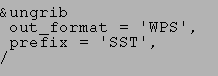
\includegraphics[width=0.45\textwidth]{ungribprefix.png}
    \caption{ \textit{\&ungrib} example.}
    \label{ungribprefix}
\end{figure}
\bigskip

\noindent Import the Variable Table for SST through a symbolic link. Type in the terminal:
\bigskip

\begin{bashcode}
ln -sf ungrib/Variable_Tables/Vtable.SST Vtable
\end{bashcode}
\bigskip

\begin{tcolorbox}[enhanced,
  grow to left by=0cm,%   equivalent to negative mdframed 'leftmargin'
  grow to right by=0cm,%  equivalent to negative mdframed 'rightmargin'
  enlarge top by=0cm,%     equivalent to mdframed 'skipabove'
  enlarge bottom by=0cm,%  equivalent to mdframed 'skipbelow'
  tcbox raise base,
  boxrule=1.0pt,
  left=18mm,
  colframe=red!50!black,coltext=red!25!black,colback=red!10!white,
  overlay={\begin{tcbclipinterior}\fill[red!75!blue!50!white] (frame.south west)
    rectangle node[text=white,font=\sffamily\bfseries\footnotesize,rotate=0] {WARNING} ([xshift=18mm]frame.north west);\end{tcbclipinterior}}]
The \textit{Vtable} is used to read the files in \textit{Grib} format. It is mandatory to use the corresponding \textit{Vtable} to the chosen 
database. You can consult them at \textit{WPS/ungrib/Variable\_Tables}.
\end{tcolorbox}
\bigskip

\noindent Create the symbolic links with the SST data through the \textit{link\_grib.csh} file:
\bigskip

\begin{bashcode}
./link_grib.csh /scratch/name.surname/Dados_CFSR/SST/*
\end{bashcode}
\bigskip

\noindent Open the \textit{qsub\_ungrib.sh} file and modify the path according to your user and type:
\bigskip

\begin{bashcode}
qsub qsub_ungrib.sh
\end{bashcode}
\bigskip

\begin{tcolorbox}[enhanced,
  grow to left by=0cm,%   equivalent to negative mdframed 'leftmargin'
  grow to right by=0cm,%  equivalent to negative mdframed 'rightmargin'
  enlarge top by=0cm,%     equivalent to mdframed 'skipabove'
  enlarge bottom by=0cm,%  equivalent to mdframed 'skipbelow'
  tcbox raise base,
  boxrule=1.0pt,
  left=18mm,
  colframe=red!50!black,coltext=red!25!black,colback=red!10!white,
  overlay={\begin{tcbclipinterior}\fill[red!75!blue!50!white] (frame.south west)
    rectangle node[text=white,font=\sffamily\bfseries\footnotesize,rotate=0] {WARNING} ([xshift=18mm]frame.north west);\end{tcbclipinterior}}]
    The \textit{qsub\_ungrib.sh} file is located in the \textit{/repository/WPS\_scripts} folder.
\end{tcolorbox}
\bigskip

\noindent Several files will be created with the initial \textit {SST:} followed by the date chosen for simulation. 
To check if everything went well, look for the message in Figure \textcolor{bleu_cite}{\ref{ungribsucess}} at the end of the file
\textit{log.out}.
\bigskip

\begin{figure}[H]
    \centering
    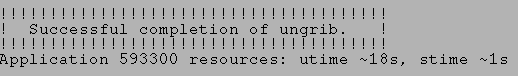
\includegraphics[width=0.45\textwidth]{qsubung.png}
    \caption{Final message in the \textit{log.out} file when running \textit{ungrib}.}
    \label{ungribsucess}
\end{figure}
\bigskip

\noindent We will proceed to the CFSR surface data. Change the \textit{prefix} in \textit{namelist.wps} (Figure \textcolor{bleu_cite}{\ref{ungribprefix}}). 
Modify \textit{SST} by \textit{SFC} and save the modification.

\bigskip

\noindent Import the CFSR \textit{Variable Table} with the symbolic link creation command:
\bigskip

\begin{bashcode}
ln -sf ungrib/Variable_Tables/Vtable.CFSR Vtable
\end{bashcode}
\bigskip

\noindent Create the symbolic links to the CFSR surface data with the command below and run \textit{ungrib} again:
\bigskip

\begin{bashcode}
./link_grib.csh /scratch/name.surname/Dados_CFSR/Surface/*
qsub qsub_ungrib.sh
\end{bashcode}
\bigskip

\noindent Look for the final message as shown in Figure \textcolor{bleu_cite}{\ref{ungribsucess}}.
\bigskip

\noindent Change the \textit{prefix} of \textit{namelist.wps} (Figure \textcolor{bleu_cite}{\ref{ungribprefix}}), replace \textit {SFC} with \textit{PRES} and save the file.
\bigskip

\noindent Create the symbolic links to the pressure data and run \textit{ungrib}:
\bigskip

\begin{bashcode}
./link_grib.csh /scratch/name.surname/Dados_CFSR/Pressure/*
qsub qsub_ungrib.sh
\end{bashcode}
\bigskip

\noindent Finally, look for the final message as identified in Figure \textcolor{bleu_cite}{\ref{ungribsucess}}. 
At the end of these steps, there will be several files with the initials \textit {SST}, \textit {PRES}, \textit {SFC} followed by the
dates of the chosen period.
\bigskip


\subsection{\textit{metgrid}}\label{metgridsecao}
\bigskip
\noindent To interpolate the data generated by \textit{ungrib.exe}, open \textit{namelist.wps} and change on the \textit{fg\_name} tab the 
names used in \textit {ungrib}. In the previous case, \textit {PRES}, \textit{SFC} and \textit{SST} were used, as in the example in 
Figure \textcolor{bleu_cite}{\ref{fgname}}:
\bigskip

\begin{figure}[H]
    \centering
    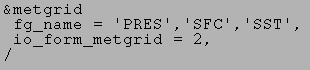
\includegraphics[width=0.5\textwidth]{fgname.png}
    \caption{\textit{\&metgrid} example.}
    \label{fgname}
\end{figure}
\bigskip

\noindent Open and then change the \textit{qsub\_metgrid.sh} file path and run:
\bigskip

\begin{bashcode}
qsub qsub_metgrid.sh
\end{bashcode}
\bigskip

\noindent Move the files generated by \textit{metgrid} (\textit {met\_em.d01*}) to the real WRF case directory:
\bigskip

\begin{bashcode}
 mv met_em.d01* /home/name.surname/WRF/test/em_real
\end{bashcode}
\bigskip


\begin{tcolorbox}[enhanced,
    grow to left by=0cm,%   equivalent to negative mdframed 'leftmargin'
    grow to right by=0cm,%  equivalent to negative mdframed 'rightmargin'
    enlarge top by=0cm,%     equivalent to mdframed 'skipabove'
    enlarge bottom by=0cm,%  equivalent to mdframed 'skipbelow'
    tcbox raise base,
    boxrule=1.0pt,
    left=18mm,
    colframe=red!50!black,coltext=red!25!black,colback=red!10!white,
    overlay={\begin{tcbclipinterior}\fill[red!75!blue!50!white] (frame.south west)
      rectangle node[text=white,font=\sffamily\bfseries\footnotesize,rotate=0] {WARNING} ([xshift=18mm]frame.north west);\end{tcbclipinterior}}]
If you are an experienced user, you can create symbolic links pointing to the \textit{met} files instead of moving them.
  \end{tcolorbox}
  \bigskip

\subsection{\textit{real}}\label{realsecao}
\bigskip

\noindent We will use the \textit{real.exe} program to generate the files that will be used in WRF. Open the file \textit{namelist.input}, 
which is in the WRF folder (\textit{/home/name.surname/WRF/test/em\_real}), and modify it according to your chosed domain and simulation time in 
\textit{namelist.wps}.
\bigskip

\noindent For the WRF to simulate the SST, it is necessary to include the following variables at the end of the section 
\textit{\&time\_control} (Figure \textcolor{bleu_cite}{\ref{timecontrolnamelist}}):
\bigskip

\begin{bashcode}
io_form_auxinput4  = 2,
auxinput4_inname   = "wrflowinp_d<domain>",
auxinput4_interval = 360,
\end{bashcode}
\bigskip

\noindent The \textit{io\_form\_auxinput4} refers to the final format of the textit{wrflowinp} file that will be generated by 
the \textit{real}. The \textit{auxinput4\_inname} is the name of the boundary condition file for SST and \textit{auxinput4\_interval} 
is the time interval, in minutes, of the boundary file.
\bigskip

\begin{figure}[H]
    \centering
    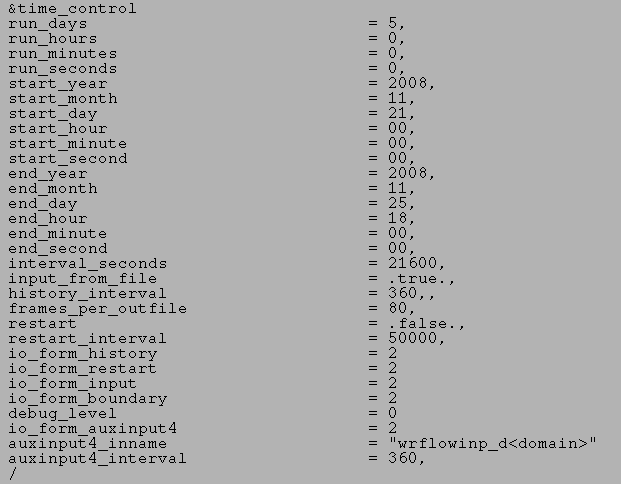
\includegraphics[width=0.70\textwidth]{namelisttimecontrol.png}
    \caption{\textit{\&time\_control} example.}
    \label{timecontrolnamelist}
\end{figure}
\bigskip

\noindent Also, in the \textit{\&physics} (Figure \textcolor{bleu_cite}{\ref{physicsnamelist}}) in the \textit{namelist.input} 
the option to update the SST:
\bigskip

\begin{bashcode}
sst_update = 1,
\end{bashcode}
\bigskip

\begin{figure}[H]
    \centering
    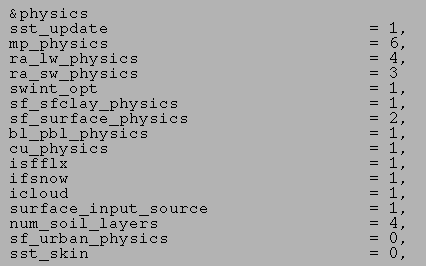
\includegraphics[width=0.70\textwidth]{physics.png}
    \caption{\textit{\&physics} example.}
    \label{physicsnamelist}
\end{figure}
\bigskip

\noindent After completing the modifications, you must use the file \textit{qsub\_real.sh} to submit the job.
The file is located in the \textit{/repository/WRF\_scripts} directory. Move the file to the \textit{em\_real} folder, change the directory 
according to your user and execute:
\bigskip

\begin{bashcode}
cd /home/name.surname/repositorio/WRF_scripts
mv qsub_real.sh /home/name.surname/WRF/test/em_real
qsub qsub_real.sh
\end{bashcode}
\bigskip

\begin{tcolorbox}[enhanced,
  grow to left by=0cm,%   equivalent to negative mdframed 'leftmargin'
  grow to right by=0cm,%  equivalent to negative mdframed 'rightmargin'
  enlarge top by=0cm,%     equivalent to mdframed 'skipabove'
  enlarge bottom by=0cm,%  equivalent to mdframed 'skipbelow'
  tcbox raise base,
  boxrule=1.0pt,
  left=18mm,
  colframe=red!50!black,coltext=red!25!black,colback=red!10!white,
  overlay={\begin{tcbclipinterior}\fill[red!75!blue!50!white] (frame.south west)
    rectangle node[text=white,font=\sffamily\bfseries\footnotesize,rotate=0] {WARNING} ([xshift=18mm]frame.north west);\end{tcbclipinterior}}]
The \textit{qsub\_real.sh} file is located in the \textit{/repository/WRF\_scripts} folder.
\end{tcolorbox}
\bigskip

\noindent To check if \textit{real} succeeded, look at the end of the \textit{log.out} file for the success message as shown 
in Figure \textcolor{bleu_cite}{\ref{realfinish}}.
\bigskip

\begin{figure}[H]
    \centering
    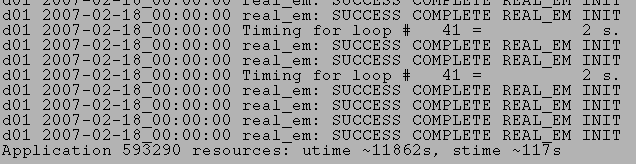
\includegraphics[width=0.70\textwidth]{realsucess.png}
    \caption{Successful completion of \textit{real}.}
    \label{realfinish}
\end{figure}
\bigskip


\noindent Upon completing \textit{real}, three files will be generated: \textit{wrfbdy\_d01}, \textit{wrfinput\_d01} and 
\textit{wrflowinp\_d01}, if you have chosen only one domain. After that, the WRF conditions are ready to be copied to your project
folder in COAWST:
\bigskip

\begin{bashcode}[fontsize=\scriptsize]
cp wrfbdy_d01 wrfinput_d01 wrflowinp_d01 /home/name.surname/COAWST/Projects/project_name
\end{bashcode}
\bigskip

\section{Using the WRF}\label{wrfsecao2}
\bigskip

\noindent With the files ready, it is possible to start the simulation of your project using only the WRF.
\bigskip

\noindent To run the simulation on the cluster, it is necessary to use the file \textit{qsub\_wrf.sh}. It is located in the 
\textit{/repository/WRF\_scripts} directory. Move the file to the WRF \textit{in\_real} folder, modify the directory according
to your user and save:
\bigskip

\begin{bashcode}
cd /home/name.surname/repositorio/WRF_scripts
mv qsub_wrf.sh /home/name.surname/WRF/test/em_real
nedit qsub_wrf.sh
\end{bashcode}
\bigskip

\noindent To start the simulation, type:
\bigskip

\begin{bashcode}
qsub qsub_wrf.sh
\end{bashcode}
\bigskip

\begin{tcolorbox}[enhanced,
  grow to left by=0cm,%   equivalent to negative mdframed 'leftmargin'
  grow to right by=0cm,%  equivalent to negative mdframed 'rightmargin'
  enlarge top by=0cm,%     equivalent to mdframed 'skipabove'
  enlarge bottom by=0cm,%  equivalent to mdframed 'skipbelow'
  tcbox raise base,
  boxrule=1.0pt,
  left=18mm,
  colframe=red!50!black,coltext=red!25!black,colback=red!10!white,
  overlay={\begin{tcbclipinterior}\fill[red!75!blue!50!white] (frame.south west)
    rectangle node[text=white,font=\sffamily\bfseries\footnotesize,rotate=0] {WARNING} ([xshift=18mm]frame.north west);\end{tcbclipinterior}}]
The \textit{qsub\_wrf.sh} file is located in the \textit{/repository/WRF\_scripts} folder.
\end{tcolorbox}
\bigskip

\noindent Follow the evolution of the job with the \textit{log.out} and \textit {log.err} files. If you want to have the information 
updated by the terminal, type:
\bigskip

\begin{bashcode}
tail -f log.out
\end{bashcode}
\bigskip
